%
% main.tex -- Paper zum Thema <quadratur>
%
% (c) 2020 Hochschule Rapperswil
%
\chapter{Gauss-Quadratur\label{chapter:quadratur}}
\lhead{Gauss-Quadratur}
\begin{refsection}
\chapterauthor{Mike Schmid}

%
% einleitung.tex -- Beispiel-File für die Einleitung
%
% (c) 2020 Prof Dr Andreas Müller, Hochschule Rapperswil
%
\section{Einleitung\label{laplace:section:einleitung}}
\rhead{Einleitung}
Lorem ipsum dolor sit amet, consetetur sadipscing elitr, sed diam
nonumy eirmod tempor invidunt ut labore et dolore magna aliquyam
erat, sed diam voluptua \cite{laplace:bibtex}.
At vero eos et accusam et justo duo dolores et ea rebum.
Stet clita kasd gubergren, no sea takimata sanctus est Lorem ipsum
dolor sit amet.

Lorem ipsum dolor sit amet, consetetur sadipscing elitr, sed diam
nonumy eirmod tempor invidunt ut labore et dolore magna aliquyam
erat, sed diam voluptua.
At vero eos et accusam et justo duo dolores et ea rebum.  Stet clita
kasd gubergren, no sea takimata sanctus est Lorem ipsum dolor sit
amet.



%
% problemstellung.tex -- Beispiel-File für die Beschreibung des Problems
%
% (c) 2020 Severin Weiss
%



\section{Motivation: Lösung einer linearen Differentialgleichung
\label{laplace:section:problemstellung}}
\rhead{Problemstellung}
Wir wollen eine Lösung $f(t)$ aus $F(s)$ der linearen Differentialgleichung 
\begin{equation}
\frac{df}{dt} + \lambda f(t) = 0, ~~mit f_{0} = f(t=0)
\end{equation}
Mit der Laplactransformation folgt
\begin{equation}
(sF(s) - f_{0}) + \lambda F(s) = 0.
\label{laplace:dgl}
\end{equation}
Die Gleichung \eqref{laplace:dgl} im Frequenzbereich kann nach $F(s)$ aufgelöst werden.
Es folgt somit
\begin{equation}
F(s) = \frac{f_{0}}{s + \lambda}
\label{laplace:F(s)}
\end{equation}
Um die Laplaceinverse von $F(s)$ zu finden existieren für gewisse Funktionstypen tabellierte zugehörige Rücktransformationen.
Für die Funktion in Gleichung \eqref{laplace:F(s)} $F(s)$ ergibt sich zum Beispiel
\begin{equation}
\mathcal{L}^{-1}\{F(s)\}=\mathcal{L}^{-1}\{\frac{f_{0}}{s+\lambda}\} = f_{0}e^{-\lambda t}
\end{equation}
Solche Tabellen sind jeweils in der Literatur zu finden, welche sich mit der Laplacetransformation beschäftigt.
Wenn für die gegebene Funktion $F(s)$ keine zugehörige Funktion tabelliert ist, muss das Integral \eqref{laplace:riemanninversionsformel} wie in der Einleitung beschrieben numerisch berechnet werden.


%
% loesung.tex -- Beispiel-File für die Beschreibung der Loesung
%
% (c) 2020 Prof Dr Andreas Müller, Hochschule Rapperswil
%
\section{Lösung
\label{fem:section:loesung}}
\rhead{Lösung}
Das gesamte Gebiet wird in Teilgebiet unterteilt und auf jedes Teilgebiet wird die Ansatzfunktion angewendet wie z.B. ein Dreieck. Wird z.B: eine lineare Ansatzfunktion gewählt sowie ein Dreieck als Teilgebiet, so hat die Ansatzfunktion die Form $u(x) = c_1 + c_2x + c_3y$. Diese Zusammensetzung ergibt sich, da der lineare Ansatz durch die Funktionswerte in den Ecken des Dreiecks bestimmt wird. In anderen Worten ausgedrückt sind die Funktionswerte in den Ecken des Teilgebiets, hier im Dreieck, die Unbekannten, die bestimmt werden müssen.
(siehe Bild \ref{fem:Approx}).\\

\begin{figure}[h!]
	\centering
	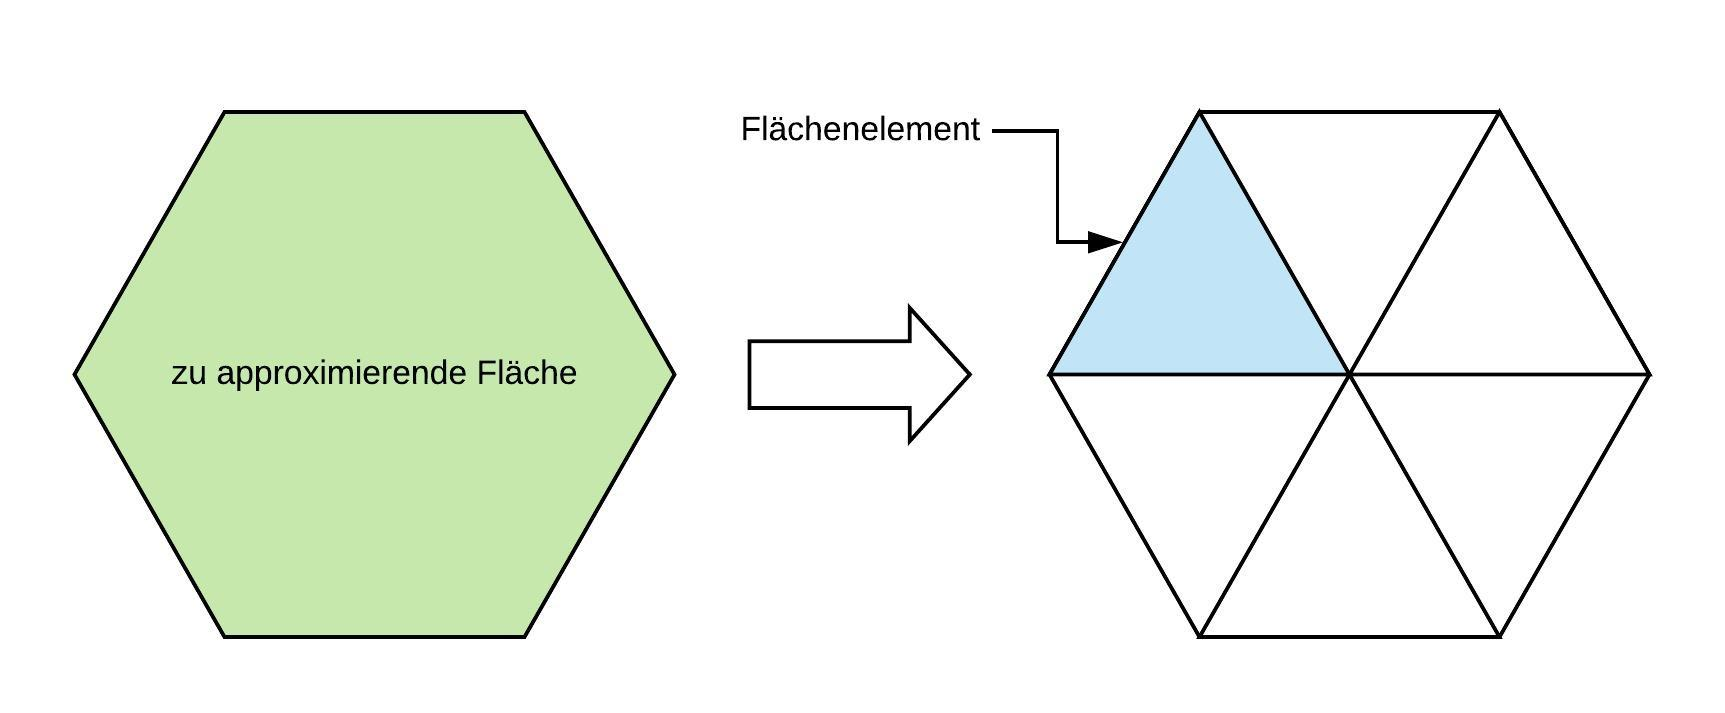
\includegraphics[scale=0.8]{papers/fem/Images/Approx.jpeg}
	\caption{Flächen- Approximation mit Dreiecks- Flächenelemente}
	\label{fem:Approx}
\end{figure}
Nochmals zur Verdeutlichung warum Ansatzfunktionen verwendet werden:
\begin{itemize}
	\item Eine einfache Formel gibt es nur auf einem kleinen Teilgebiete
	\item In dem Teilgebiet ist die Formel sehr einfach zu berechnen wie z.B. eine lineare Funktion die durch Koeffizienten bestimmt wird.
\end{itemize}
Als Standardverfahren in der Ebene haben sich Flächenelement wie Dreiecken oder Parallelogramme bewährt. Die Wahl der  der Flächen- bzw. Gebiet- Elementen sollte so erfolgen, dass diese die zu approximierende Fläche möglichst gut nachbildet bzw. approxmimiert wird.

Um möglichst einfach darzustellen, wie das Verfahren der Finiten Elemente vonstatten geht, wurde auf eine einfache Approximation mit Einheitsdreiecken und einem linearen Ansatz gewählt. 

\subsection{Vorbereitung}

Damit die Integration über das gewählte Teilgebiet bzw. Flächenelement einfacher fällt, wird als Vorbereitung im entsprechenden Fall das gewählte Flächenelement in ein Einheitsdreieck oder in ein Eineheitsparallelogramm transformiert. Ein Dreieck oder Parallelogramm stellt eine Formfunktion dar, über die die gewählte Fläche bzw. Teilgebiet berechnet werden kann. Die gewählte Formfunktion eines Teilgebietes z.B. integrieren des Gebietes über ein Dreieck oder Pallelogramm,  bringt auch den Vorteil, dass die gewählten Formfunktionen gleich behandelt werden können. \\
Das allgemeine Dreieck in allgemeiner Lage mit den Eckpunkten $P_1(x_1, y_1$), $ P_2(x_2, y_2)$ und $P3(x_3,y_3)$ kann mit Hilfe der linearen Transformation \eqref{fem:linTransformation}

\begin{equation}
	\begin{split}
		x = x_1 + (x_2 - x_1)\xi + (x_3 - X_1)\eta \\
		y = y_1 + (y_2 - y_1)\xi + (y_3 - y_1)\eta
		\label{fem:linTransformation}
	\end{split}
\end{equation}
in das einfachere Gebiet nämlich dem gleichschenklig rechtwinklige Einheitsdreieck mit Kathetenlänge 1 überführt werden.


\begin{figure}[h!]
	\centering
	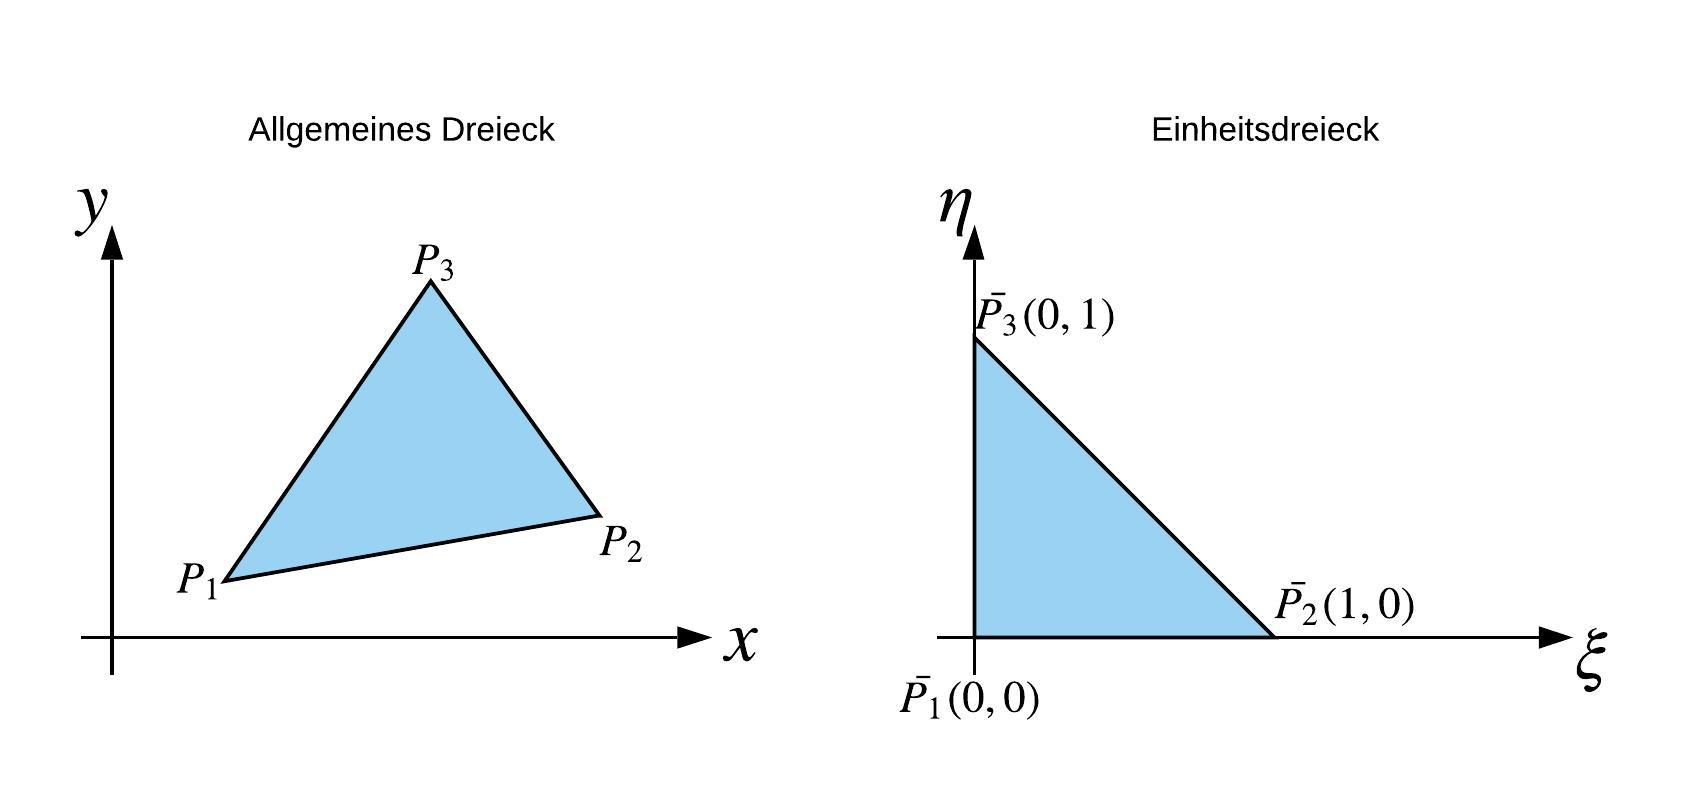
\includegraphics[scale=0.8]{papers/fem/Images/Dreiecke.jpeg}
	\caption{Transformation in ein Einheitsdreieck}
	\label{fig:schemNMR_vorlage}
\end{figure}
Die Transformation soll untern den elementaren Regeln der Analysis vorgenommen werden. Nun ist das Flächenelement $dx \, dy$ mit Hilfe der Jacobi Determinante \eqref{fem:JocobiDeterminante} der Transformation zu ersetzen durch \eqref{fem:newTransformation}.

\begin{equation}
J % 
=
\begin{bmatrix}
    \frac{\partial x}{\partial \xi} &  \frac{\partial x}{\partial \eta}     \\
   \frac{\partial y}{\partial \xi}  &  \frac{\partial y}{\partial \eta}     
\end{bmatrix}
= 
\begin{bmatrix}
    x_2 - x_1  &  x_3 -x_1      \\
    y_2 - y_1  &  y_3 - y_1      
\end{bmatrix} 
	\label{fem:JocobiDeterminante}
\end{equation}
Die Determinante dieser Jacobi- Matrix ergibt
\begin{equation}
	det(J) = x_1 \cdot y_2 - 2 \cdot x_1 \cdot y_1 + x_2 \cdot y_1 + x_1\cdot y_3 + x_3 \cdot y_1 - x_2 \cdot y_3 - x_3 \cdot y_2
	\label{fem:JocobiDetBerechnet}
\end{equation}
\begin{equation}
			dy \, dy = det(J) \, d\xi \, d\eta
			\label{fem:newTransformation}
\end{equation}
Die Jacobi- Determinante entspricht der doppelten Fläche des Dreiecks. Die partiellen Ableitungen werden gemäss der Kettenregel zu 
%\begin{equation}
%			\begin{aligned}
%			u_x = u_{\xi} \xi_x + u_{\eta} \eta_x \\
%			u_y = u_{\xi} \xi_y + u_{\eta} \eta_y 
% 			\end{aligned}
%			\label{fem:newKoordinate}
%\end{equation}
\begin{equation}
\begin{split}
	\frac{\partial u}{\partial x} = \frac{\partial u}{\partial \xi} \, \frac{\partial \xi}{\partial x} + \frac{\partial u}{\partial \eta} \, \frac{\partial \eta}{\partial x} \\
	\frac{\partial u}{\partial y} = \frac{\partial u}{\partial \xi} \, \frac{\partial \xi}{\partial y} + \frac{\partial u}{\partial \eta} \, \frac{\partial \eta}{\partial y}
	\end{split}
\end{equation}
Auf Grund der linearen Transformation \eqref{fem:linTransformation} ergeben sich nach der partieller Differentiation der beiden Beziehungen nach $x$ zunächst

\begin{equation}
			\begin{aligned}
			1  = (x_2 -x_1) \, \eta_x + (x_3 -x_1) \, \eta_x \\
			0 = (y_2 -y_1) \, \eta_x + (y_3 -y_1) \, \eta_x \\
			 \end{aligned}
\end{equation}
Nach Auflösung  der beiden Gleichungen nach $\xi_x$ und $\eta_x$ ergibt sich

\begin{equation}
			\xi_x = \frac{y_3 - y_1}{J} \quad \eta_x = -\frac{y_2 - y_1}{J}
\end{equation}
Analog nach der partiellen Ableitung nach $y$ erhält man

\begin{equation}
			\xi_y = \frac{x_3 - x_1}{J} \quad \eta_y = -\frac{x_2 - x_1}{J}
\end{equation}

\subsection{Schritt 1 Minimalproblem bilden}

Analog bei den Finiten Elementen im 1 dimensionale Raum, muss auch die DGL in der Ebene zuerst in ein äquivalentes Minimalproblem übersetzt werden. Das Minimalproblem für FEM in einer Dimension hatte die Form

\begin{equation}
			\int_0^1 u \textcolor{red}{'} (x)^2 - \lambda \, u(x)^2 dx \,dy
			\label{fem:Minimal1D}
\end{equation}
Im Unterschied zu den mehrdimensionale Form wird anstatt der einfachen Ableitungt der Laplace Operator verwendet der zugleich zweifache Differenziebarkeit von der Ansatzfunktion $u(x)$ fordert. Zudem wird nicht mehr über eine Strecke integriert sondern nun über ein Gebiet $\Omega$ was gleichbedeutend für eine Integration über eine Fläche steht.

\begin{equation}
			\int_{\Omega} (\textcolor{red}{\nabla} u)^2 - \lambda u^2 dx \, dy
			\label{fem:Minimal2D}
\end{equation}
Der Integrationsterm \ref{fem:Minimal2D} wird gemäss der Summenregel in 2 Terme zerlegt nämlich 

\begin{equation}
			\int_{\Omega} (\nabla u)^2 \, dx \, dy - \lambda \int_{\Omega} u^2 dx \, dy
			\label{fem:Minimal2D2Term}
\end{equation}
Nun ist die Bildung des Minimalproblems abgeschlossen. In einem nächsten Schritt sollen je nach Ausgangslage, gewisse Vorbereitungen getroffen werden die in dem folgenden Abschnitt erläutert werden.

\subsection{ 2. Ansatzfunktionen auf Lösung approximieren}

%Als Ansatzfunktionen stehen diverse Standard- Funktionen in der Ebene zur Verfügung. Sie reichen von einfacheren linearen Termen bishinzu quadratischen oder noch höheren Funktions- Ordnungen. Als Standardverfahren in der Ebene haben sich Flächenelement wie Dreicecken oder Parallelogrammebewährt. Die Wahl der  der Flächen- Elementen sollte so erfolgen, dass diese die zu approximierende Fläche möglichst gut nachbildet bzw. approxmimiert wird.

%Die Wahl der Art der Approximationsfunktion wie linear oder quadratisch wird in xXx behandelt.

%Um möglichst einfach darzustellen, wie das Verfahren der Finiten Elemente vonstatten geht, wurde auf eine einfache Approximation mit Einheitsdreiecken und einem linearen Ansatz gewählt. 


Die lineare Ansatzfunktion hat die folgende Form

\begin{equation}
u(x,y) = c_1 + c_2x + c_3y
\label{fem:equationSchwarzLinear}
\end{equation}
Die Ansatzfunktion \ref{fem:equationSchwarzLinear} kann somit direkt in das Minimalproblem \ref{fem:Minimal2D} eingesetzt werden. Ziel ist es, dass die unbekannten Koeffizienten $c_1, c_2 \, $und$ \, c_3$ anhand dieses Verfahrens bestimmt werden.

Das Minimalproblem beinhaltet jedoch noch nicht die Formfunktion des Flächenelements. Diese wird in das Gebietsintegral des Minimalproblem eingesetzt sprich $\int_{\Omega}$ wird durch das folgende Flächenelement bzw. Flächenintegral ersetzt. Wie bereits ankeündigt wird das Einheitsdreieck für dieses Beispiel verwendet.

\begin{equation}
\int_a^b \int_c^{d-(d-c)(x-a)/(b-a)} f(x,y) \, dx\,dy
\label{fem:FlaecheDreieck}
\end{equation}
Schlussendlich ergibt das Einsatzen der Ansatzfunktion und des Flächenintegrals dann folgenden Ausdruck.

\begin{equation}
\int_a^b \int_c^{d-(d-c)(x-a)/(b-a)} c_1 + c_2x + c_3y \, dx \, dy
\label{fem:MinimalproblemElement}
\end{equation}
Wichtig zu verstehen ist, dass dieses Minimalproblem bzw. der Ausdruck \ref{fem:MinimalproblemElement} auf jedes Flächenelement angewendet wird. Sprich jedes Element hat einn zugehöriges Minimalproblems. Als Beispiel kann vorgestellt werden, dass wenn ein Rechteck mit zwei Dreiecken approximiert wird, das Minimalproblem \ref{fem:MinimalproblemElement} auf jedes der beiden Dreiecke angewendet wird. Je feiner die Auflösung, desto grösser das Gleichungs- System das Schluss endlich gelöst werden muss.

Nun kann der erste Teil der Berechnung beginnen. Die partielle Ableitung nach dergewählten linearen Funktion $f(u)$ erigbt das Resultat

\begin{equation}
	\nabla u = 	
	\left[ \begin{array}{r}
	c_2  \\
	c_3 \\
	\end{array}\right]
	\label{fem:equationSchwarzquadratischP}
\end{equation} 

\subsubsection{Gleichungssystem aufstellen }

Für jedes Flächenelement gilt die Gleichung \ref{fem:MinimalproblemElement}. Nun müssen alle diese Elemente in eine Matrix umgeschrieben werden die sich wie folgt zusammensetzen lässt.

\begin{equation}
			\underbrace{ \int_{\Omega} (\nabla u)^2 dx \, dy} \, -  \, \underbrace{\lambda \int_{\Omega} u^2 dx \,dy}
			\label{fem:Minimal2TermLinAlg}
\end{equation}


\begin{equation}
			c^t Ac \, - \, \lambda c^t Bc
			\label{fem:Minimal2LinAlg}
\end{equation}
Die Matrix $A$ wird gebildet durch die Teilmatrizen eines jeden Flächenelements. Die Teilmatrix eines Flächenelements besteht  aus dem Integral des 1. Terms von \ref{fem:Minimal2TermLinAlg} 

\begin{equation}
			\int_a^b \int_c^{d-(d-c)(x-a)/(b-a)} \left( \begin{array}{c} c_2 \\ c_3\\	
\end{array} \right)^2 dx \, dy
			\label{fem:Minimal2LinAlgA}
\end{equation}
was dann zu der entsrechenden Teilmatrix eines Dreiecks führt

\begin{equation}
	\left( \begin{array}{cc}
	c_2^2 \int_{\Omega} 1 dx \, dy & 0  \\ 
	0 & c_3^2 \int_{\Omega} 1 dx \, dy  \\
	\end{array}\right)
	\label{fem:TeilmatrixA}
\end{equation}
und wird dann in die Matrix $A $eingefügt bzw. zusammengefasst, dass  somti sämtliche Teilmatrizen aller Flächenelemente in der Matrix $A$ vorhanden sind. Eine jede Farbe soll veranschaulichen, dass dies ein Dreieck- Flächenelement darstellt.

\begin{equation}
 A = \begin{pmatrix} 0 & 0 & \hdotsfor{4} & 0 \\
	0 & \textcolor{green}{ c_2^2 \int_{\Omega} 1 dx \, dy }& \vdots & 0 & \vdots & & \vdots \\
	\vdots & \vdots & \textcolor{green}{c_3^2 \int_{\Omega} 1 dx \, dy }& 0 & \vdots  & & \\
	\vdots & \vdots & 0 & \ddots & \textcolor{red}{ c_2^2 \int_{\Omega} 1 dx \, dy }& & \\
	\vdots & \vdots & 0 & 0 & 0 & \textcolor{red}{c_3^2 \int_{\Omega} 1 dx \, dy} & \\
	0 & \hdotsfor{2} & 0 &  & & &  \ddots  \\
	\end{pmatrix}
	\label{fem:MatrixA}
\end{equation}
Die Matrix $A$ ist nun bekannt. Es fehlt jedoch noch die Matrix $B$, um das Gleichungs-System zu komplettieren. Die Matrix $B$ wird nun wie folgt definiert. Um die folgende Form zu erhalten muss lediglich der rechte Term von \ref{fem:Minimal2D2Term} für die einzelne Koeffizienten berechnet werden was dann den folgenden Ausdruck ergibt

\begin{equation}
			\int_a^b \int_c^{d-(d-c)(x-a)/(b-a)} \textcolor{cyan}{c_0^2} + \textcolor{blue}{c_1^2 x^2} + \textcolor{red}{c_2^2 y^2} + \textcolor{green}{2 c_0 c_1 x} + \textcolor{orange}{2 c_0 c_2 y} +\textcolor{purple}{ 2 c_1 c_2 xy} \, dx \, dy
			\label{fem:Minimal2LinAlgB}
\end{equation}
Nun soll dies wieder in die Matrix- Schreibweise übertragen werden was dann eine Teilmatrix $B$ eines Dreickes entspricht

\begin{equation}
 B = \left( \begin{array}{ccc}
	\textcolor{cyan}{- \lambda \int_{\Omega} 1} &  \textcolor{green}{- \lambda \int_{\Omega} x} & \textcolor{orange}{- \lambda \int_{\Omega} y}  \\
	\textcolor{green}{- \lambda \int_{\Omega}x} & \textcolor{blue}{- \lambda \int_{\Omega} x^2} &  \textcolor{purple}{- \lambda \int_{\Omega} xy} \\
	\textcolor{orange}{- \lambda \int_{\Omega} y} & \textcolor{purple}{- \lambda \int_{\Omega} xy} & \textcolor{red}{ - \lambda \int_{\Omega} y^2} \\
	\end{array}\right)
	\label{fem:MatrixB}
\end{equation}
Diese Teilmatrix $B$ eines jeden Flächenelements wird dann wieder analog der Matrix $A$ in eine Matrix $B$ eingesetzt, so dass diese dann alle Teilmatrizen aller Dreieck-  Flächenstücke enthält.


\subsection{Schritt 3 Minimalprinizip anwenden auf Approximation}

Nun folgt der nächste Schritt nämlich das Minimieren des quadratischen Ausdrucks
\begin{equation}
	c^t Ac - c^t \lambda Bc
\end{equation}
Was so viel bedeutet wie nach den Koeffizienten $c_k$ ableiten was für den  für 1. Term
\begin{equation}
	\nabla c^t Ac = 2Ac
\end{equation}
ergibt und für den 2. Term den Ausdruck

\begin{equation}
	\nabla c^t \lambda Bc = 2\lambda Bc
\end{equation}
Diese Ableitungen erscheinen nicht gerade ersichtlich insbesondere der Faktor 2. 

Das ableiten im 1- Dimensionalen Raum ergibt nach der klassichen Analysis

\begin{equation}
	\frac{d}{dx} ax^2 = 2ax
\end{equation}
Um die Ableitung in einem n-Dimensionalen, quadratischen Matrix vorzunehmen muss diese erst in einen Summennotation umgeschrieben werden wie folgt

\begin{equation}
			x^tAx, x \in \mathbb{R}^n
\end{equation}
Zu erkennen ist, dass nach der Ableitung von $x$ die Produkt- Regel zum tragen kommt. 

\begin{equation}
	\sum_{i,j} \frac{\partial x_i}{\partial x_n} a_{ij} x_j + \sum_{i,j} x_i a_{ij} \frac{\partial x_j}{\partial x_n}
\end{equation}
Dies kann vereinfacht werden anhand der folgenden Kürzungs- Berechnung:

\begin{equation}
	\sum_{j} a_{nj} x_j + \sum_{i,j} x_i a_{in} = \sum_{j} a_nj x_j + \sum_{\textcolor{red}{\not{j}} i} a_{n \textcolor{red}{\not{j}} i} x_{\textcolor{red}{\not{j}} i} = 2(Ax)_n
\end{equation}

\subsection{Schritt 5 Gleichungssystem aufstellen}
Nun kann das Gleichungssystem aufgestellt werden.
\begin{equation}
	2Ac - 2\lambda Bc = 0 \Rightarrow (A-\lambda B)c = 0
	\label{fem:GLLang}
\end{equation}
Durch das umschreiben der Gleichung \ref{fem:GLLang} ist ersichtlich, dass es sich um ein Eigenwertproblem für die Matrix $B^{-1}A$ handelt.

\begin{equation}
		B^{-1}Ac = \lambda c
 \end{equation}
 Dieses kann z.B. durch das Jacobi Verfahren, beschrieben im Kapitel 6.4 gelöst werden.
 
\subsection{Andere lineare Ansatzfunktionen
\label{fem:subsection:Ansatzfunktionen}}

Neben dem durchgerechneten Beispiel des Einheitsdreiecks kann auch eine andere Formfunktion verwendet werden. Die folgende Formfunktion gilt für den linearen Ansatz eines Parallelogramms.

\begin{equation}
	u(x,y) = c_1 + c_2 x + c_3 y + c_4 xy
\end{equation} 


\subsubsection{Quadratischer Ansatz
\label{fem:subsection:bonorum}}

Der Vorteil des quadratischen Ansatzes liegt darin, dass die Freiheitsgeraden erhöht werden. Somit kann unter umständen eine bessere Approximation erreicht werden.
Zu beachten ist allerdings, dass diese die Matrix enorm aufblasen bzw. vergrössern und dann mehr Ressourcen in Anspruch nehmen, um die Matrix bzw. die Eigen werte zu berechnen.

In der Gleichung \ref{fem:equationSchwarzquadratischD}  ist der Ansatz für das Einheitsdreieck gegeben. Und in der Gleichung \ref{fem:equationSchwarzquadratischP} der quadratische Ansatz für ein Einheitsparallelogramm.

\begin{equation}
	u(x,y) = c_1 + c_2 x + c_3 y + c_4 x^2 + c_5 xy + c_6 y^2
	\label{fem:equationSchwarzquadratischD}
\end{equation}

\begin{equation}
	u(x,y) = c_1 + c_2 x + c_3 y + c_4 x^2 + c_5 xy + c_6 y^2 + c_7 x^2y + c_8 xy^2
	\label{fem:equationSchwarzquadratischP}
\end{equation} 




%
% problemstellung.tex -- Beispiel-File für die Beschreibung des Problems
%
% (c) 2020 Prof Dr Andreas Müller, Hochschule Rapperswil
%
\section{Folgerungen
\label{ew:section:folgerungen}}
\rhead{Folgerungen}
Sed ut perspiciatis unde omnis iste natus error sit voluptatem
accusantium doloremque laudantium, totam rem aperiam, eaque ipsa
quae ab illo inventore veritatis et quasi architecto beatae vitae
dicta sunt explicabo. Nemo enim ipsam voluptatem quia voluptas sit
aspernatur aut odit aut fugit, sed quia consequuntur magni dolores
eos qui ratione voluptatem sequi nesciunt. Neque porro quisquam
est, qui dolorem ipsum quia dolor sit amet, consectetur, adipisci
velit, sed quia non numquam eius modi tempora incidunt ut labore
et dolore magnam aliquam quaerat voluptatem. Ut enim ad minima
veniam, quis nostrum exercitationem ullam corporis suscipit laboriosam,
nisi ut aliquid ex ea commodi consequatur? Quis autem vel eum iure
reprehenderit qui in ea voluptate velit esse quam nihil molestiae
consequatur, vel illum qui dolorem eum fugiat quo voluptas nulla
pariatur?

\subsection{De finibus bonorum et malorum
\label{ew:subsection:malorum}}
At vero eos et accusamus et iusto odio dignissimos ducimus qui
blanditiis praesentium voluptatum deleniti atque corrupti quos
dolores et quas molestias excepturi sint occaecati cupiditate non
provident, similique sunt in culpa qui officia deserunt mollitia
animi, id est laborum et dolorum fuga. Et harum quidem rerum facilis
est et expedita distinctio. Nam libero tempore, cum soluta nobis
est eligendi optio cumque nihil impedit quo minus id quod maxime
placeat facere possimus, omnis voluptas assumenda est, omnis dolor
repellendus. Temporibus autem quibusdam et aut officiis debitis aut
rerum necessitatibus saepe eveniet ut et voluptates repudiandae
sint et molestiae non recusandae. Itaque earum rerum hic tenetur a
sapiente delectus, ut aut reiciendis voluptatibus maiores alias
consequatur aut perferendis doloribus asperiores repellat.




\printbibliography[heading=subbibliography]
\end{refsection}
